\section{Adaptive Huffmancoding met sliding window}

\subsection{Downdate}
De \emph{downdate}-procedure is gebaseerd op de \emph{Adaptive Update}-procedure, maar dan omgekeerd, hetzelfde geldt voor de procedure om de wisseltop te bepalen. Indien er een top gewicht $0$ bereikt wordt deze verwijderd uit de boom. Nadat deze top verwijderd is is het belangrijk dat er gecontroleerd wordt dat \texttt{nng} de broer is van de top met het laagste gewicht en laagste ordernummer\footnote{Er wordt aangenomen dat de ordenummers op aflopende volgorde gesorteerd zijn; de wortel heeft het hoogste ordernummer.}. Indien dit niet het geval is zal de boom in een ongeldige toestand terecht komen wanneer een volgend karakter verwijderd wordt. 

\subsection{Grootte van het sliding window}
Knuth beschrijft in zijn paper \cite{knuthhuffman} wat de optimale windowgroottes zijn op pagina 180. Volgens de tabel ligt deze waarde op \texttt{$1\ 250$}, maar zelf heb ik ook een aantal experimenten uitgevoerd om zo voor tekstuele data de optimale windowgrootte te bepalen. Uit deze experimenten bleek dat de optimale windowgrootte veel hoger ligt, namelijk op \texttt{$15\ 000$}. Een verklaring hiervoor is dat Knuth wellicht zeer kleine teksten ge\"encodeerd heeft. De grafiek in figuur \ref{fig:sliding-windowsizes} toont de compressieratio's\footnote{Compressieratio wordt gedefinieerd als $(\frac{c}{o})$ met $c,o$ respectievelijk de groottes van de gecomprimeerde tekst en de originele tekst, uitgedrukt in bytes.} De tests werden steeds uitgevoerd op 6 fragmenten uit de King James Bible \cite{gutenbergbible} met verschillende lengtes. De bestandsgroottes van deze bestanden zijn respectievelijk $\SI{100}{\byte}, \SI{1}{\kibi\byte}, \SI{10}{\kibi\byte}, \SI{100}{\kibi\byte}, \SI{1}{\mebi\byte}$ en $\SI{10}{\mebi\byte}$. Deze bestanden werden ge\"encodeerd voor verschillende windowgroottes, waarna het gemiddelde van de compressieratio's per windowgrootte werd bepaald en in de grafiek werd geplot. Het minimum van de grafiek bevindt zich in de buurt van \SI{15000}{\byte}.

\begin{figure}[h]
	\centering
	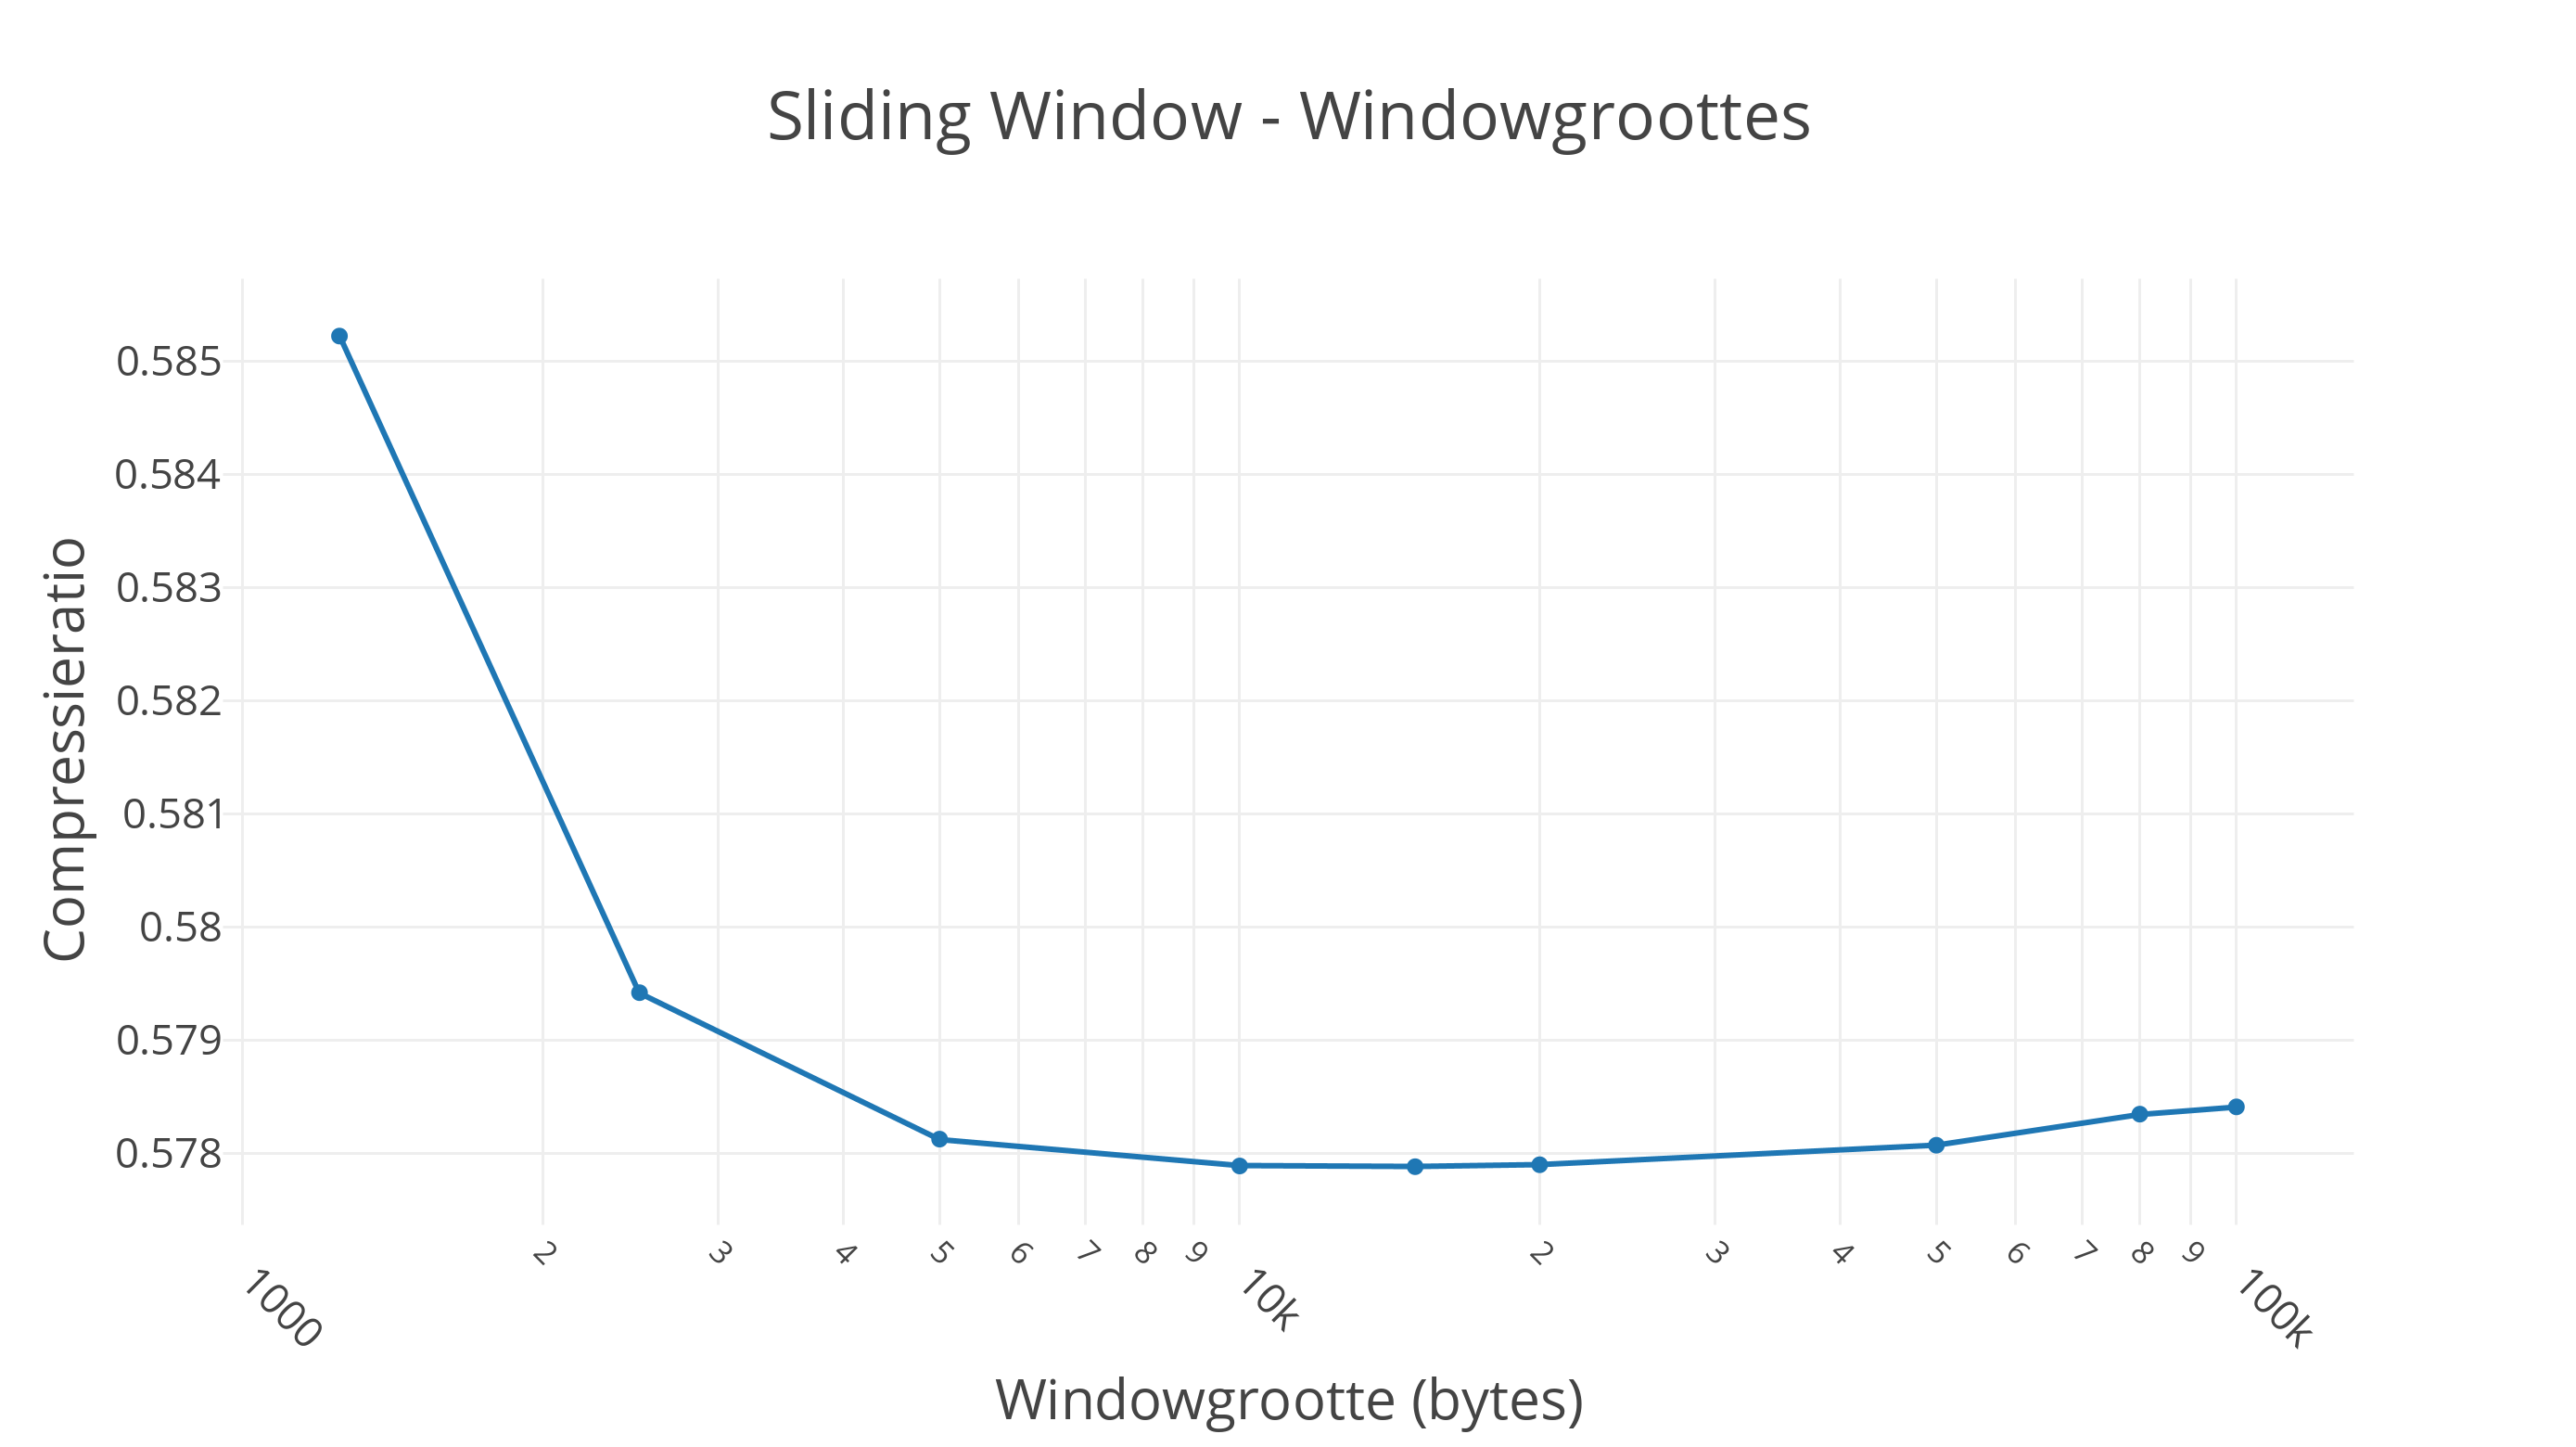
\includegraphics[width=0.9\linewidth]{resources/sliding-window.png}
	\label{fig:sliding-windowsizes}
	\caption{Vergelijking tussen verschillende windowgroottes}
\end{figure}